\documentclass[1p]{elsarticle_modified}
%\bibliographystyle{elsarticle-num}

%\usepackage[colorlinks]{hyperref}
%\usepackage{abbrmath_seonhwa} %\Abb, \Ascr, \Acal ,\Abf, \Afrak
\usepackage{amsfonts}
\usepackage{amssymb}
\usepackage{amsmath}
\usepackage{amsthm}
\usepackage{scalefnt}
\usepackage{amsbsy}
\usepackage{kotex}
\usepackage{caption}
\usepackage{subfig}
\usepackage{color}
\usepackage{graphicx}
\usepackage{xcolor} %% white, black, red, green, blue, cyan, magenta, yellow
\usepackage{float}
\usepackage{setspace}
\usepackage{hyperref}

\usepackage{tikz}
\usetikzlibrary{arrows}

\usepackage{multirow}
\usepackage{array} % fixed length table
\usepackage{hhline}

%%%%%%%%%%%%%%%%%%%%%
\makeatletter
\renewcommand*\env@matrix[1][\arraystretch]{%
	\edef\arraystretch{#1}%
	\hskip -\arraycolsep
	\let\@ifnextchar\new@ifnextchar
	\array{*\c@MaxMatrixCols c}}
\makeatother %https://tex.stackexchange.com/questions/14071/how-can-i-increase-the-line-spacing-in-a-matrix
%%%%%%%%%%%%%%%

\usepackage[normalem]{ulem}

\newcommand{\msout}[1]{\ifmmode\text{\sout{\ensuremath{#1}}}\else\sout{#1}\fi}
%SOURCE: \msout is \stkout macro in https://tex.stackexchange.com/questions/20609/strikeout-in-math-mode

\newcommand{\cancel}[1]{
	\ifmmode
	{\color{red}\msout{#1}}
	\else
	{\color{red}\sout{#1}}
	\fi
}

\newcommand{\add}[1]{
	{\color{blue}\uwave{#1}}
}

\newcommand{\replace}[2]{
	\ifmmode
	{\color{red}\msout{#1}}{\color{blue}\uwave{#2}}
	\else
	{\color{red}\sout{#1}}{\color{blue}\uwave{#2}}
	\fi
}

\newcommand{\Sol}{\mathcal{S}} %segment
\newcommand{\D}{D} %diagram
\newcommand{\A}{\mathcal{A}} %arc


%%%%%%%%%%%%%%%%%%%%%%%%%%%%%5 test

\def\sl{\operatorname{\textup{SL}}(2,\Cbb)}
\def\psl{\operatorname{\textup{PSL}}(2,\Cbb)}
\def\quan{\mkern 1mu \triangleright \mkern 1mu}

\theoremstyle{definition}
\newtheorem{thm}{Theorem}[section]
\newtheorem{prop}[thm]{Proposition}
\newtheorem{lem}[thm]{Lemma}
\newtheorem{ques}[thm]{Question}
\newtheorem{cor}[thm]{Corollary}
\newtheorem{defn}[thm]{Definition}
\newtheorem{exam}[thm]{Example}
\newtheorem{rmk}[thm]{Remark}
\newtheorem{alg}[thm]{Algorithm}

\newcommand{\I}{\sqrt{-1}}
\begin{document}

%\begin{frontmatter}
%
%\title{Boundary parabolic representations of knots up to 8 crossings}
%
%%% Group authors per affiliation:
%\author{Yunhi Cho} 
%\address{Department of Mathematics, University of Seoul, Seoul, Korea}
%\ead{yhcho@uos.ac.kr}
%
%
%\author{Seonhwa Kim} %\fnref{s_kim}}
%\address{Center for Geometry and Physics, Institute for Basic Science, Pohang, 37673, Korea}
%\ead{ryeona17@ibs.re.kr}
%
%\author{Hyuk Kim}
%\address{Department of Mathematical Sciences, Seoul National University, Seoul 08826, Korea}
%\ead{hyukkim@snu.ac.kr}
%
%\author{Seokbeom Yoon}
%\address{Department of Mathematical Sciences, Seoul National University, Seoul, 08826,  Korea}
%\ead{sbyoon15@snu.ac.kr}
%
%\begin{abstract}
%We find all boundary parabolic representation of knots up to 8 crossings.
%
%\end{abstract}
%\begin{keyword}
%    \MSC[2010] 57M25 
%\end{keyword}
%
%\end{frontmatter}

%\linenumbers
%\tableofcontents
%
\newcommand\colored[1]{\textcolor{white}{\rule[-0.35ex]{0.8em}{1.4ex}}\kern-0.8em\color{red} #1}%
%\newcommand\colored[1]{\textcolor{white}{ #1}\kern-2.17ex	\textcolor{white}{ #1}\kern-1.81ex	\textcolor{white}{ #1}\kern-2.15ex\color{red}#1	}

{\Large $\underline{12n_{0833}~(K12n_{0833})}$}

\setlength{\tabcolsep}{10pt}
\renewcommand{\arraystretch}{1.6}
\vspace{1cm}\begin{tabular}{m{100pt}>{\centering\arraybackslash}m{274pt}}
\multirow{5}{120pt}{
	\centering
	\includegraphics[width=112pt]{../../../GIT/diagram.site/Diagrams/png/2922_12n_0833.png}\\
\ \ \ A knot diagram\footnotemark}&
\allowdisplaybreaks
\textbf{Linearized knot diagam} \\
\cline{2-2}
 &
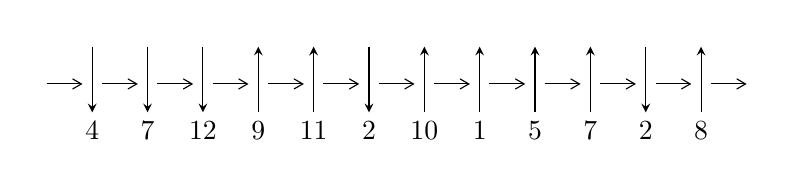
\begin{tikzpicture}[x=20pt, y=17pt]
	% nodes
	\node (C0) at (0, 0) {};
	\node (C1) at (1, 0) {};
	\node (C1U) at (1, +1) {};
	\node (C1D) at (1, -1) {4};

	\node (C2) at (2, 0) {};
	\node (C2U) at (2, +1) {};
	\node (C2D) at (2, -1) {7};

	\node (C3) at (3, 0) {};
	\node (C3U) at (3, +1) {};
	\node (C3D) at (3, -1) {12};

	\node (C4) at (4, 0) {};
	\node (C4U) at (4, +1) {};
	\node (C4D) at (4, -1) {9};

	\node (C5) at (5, 0) {};
	\node (C5U) at (5, +1) {};
	\node (C5D) at (5, -1) {11};

	\node (C6) at (6, 0) {};
	\node (C6U) at (6, +1) {};
	\node (C6D) at (6, -1) {2};

	\node (C7) at (7, 0) {};
	\node (C7U) at (7, +1) {};
	\node (C7D) at (7, -1) {10};

	\node (C8) at (8, 0) {};
	\node (C8U) at (8, +1) {};
	\node (C8D) at (8, -1) {1};

	\node (C9) at (9, 0) {};
	\node (C9U) at (9, +1) {};
	\node (C9D) at (9, -1) {5};

	\node (C10) at (10, 0) {};
	\node (C10U) at (10, +1) {};
	\node (C10D) at (10, -1) {7};

	\node (C11) at (11, 0) {};
	\node (C11U) at (11, +1) {};
	\node (C11D) at (11, -1) {2};

	\node (C12) at (12, 0) {};
	\node (C12U) at (12, +1) {};
	\node (C12D) at (12, -1) {8};
	\node (C13) at (13, 0) {};

	% arrows
	\draw[->,>={angle 60}]
	(C0) edge (C1) (C1) edge (C2) (C2) edge (C3) (C3) edge (C4) (C4) edge (C5) (C5) edge (C6) (C6) edge (C7) (C7) edge (C8) (C8) edge (C9) (C9) edge (C10) (C10) edge (C11) (C11) edge (C12) (C12) edge (C13) ;	\draw[->,>=stealth]
	(C1U) edge (C1D) (C2U) edge (C2D) (C3U) edge (C3D) (C4D) edge (C4U) (C5D) edge (C5U) (C6U) edge (C6D) (C7D) edge (C7U) (C8D) edge (C8U) (C9D) edge (C9U) (C10D) edge (C10U) (C11U) edge (C11D) (C12D) edge (C12U) ;
	\end{tikzpicture} \\
\hhline{~~} \\& 
\textbf{Solving Sequence} \\ \cline{2-2} 
 &
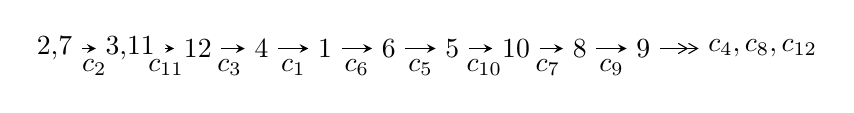
\begin{tikzpicture}[x=23pt, y=7pt]
	% node
	\node (A0) at (-1/8, 0) {2,7};
	\node (A1) at (17/16, 0) {3,11};
	\node (A2) at (17/8, 0) {12};
	\node (A3) at (25/8, 0) {4};
	\node (A4) at (33/8, 0) {1};
	\node (A5) at (41/8, 0) {6};
	\node (A6) at (49/8, 0) {5};
	\node (A7) at (57/8, 0) {10};
	\node (A8) at (65/8, 0) {8};
	\node (A9) at (73/8, 0) {9};
	\node (C1) at (1/2, -1) {$c_{2}$};
	\node (C2) at (13/8, -1) {$c_{11}$};
	\node (C3) at (21/8, -1) {$c_{3}$};
	\node (C4) at (29/8, -1) {$c_{1}$};
	\node (C5) at (37/8, -1) {$c_{6}$};
	\node (C6) at (45/8, -1) {$c_{5}$};
	\node (C7) at (53/8, -1) {$c_{10}$};
	\node (C8) at (61/8, -1) {$c_{7}$};
	\node (C9) at (69/8, -1) {$c_{9}$};
	\node (A10) at (11, 0) {$c_{4},c_{8},c_{12}$};

	% edge
	\draw[->,>=stealth]	
	(A0) edge (A1) (A1) edge (A2) (A2) edge (A3) (A3) edge (A4) (A4) edge (A5) (A5) edge (A6) (A6) edge (A7) (A7) edge (A8) (A8) edge (A9) ;
	\draw[->>,>={angle 60}]	
	(A9) edge (A10);
\end{tikzpicture} \\ 

\end{tabular} \\

\footnotetext{
The image of knot diagram is generated by the software ``\textbf{Draw programme}" developed by Andrew Bartholomew(\url{http://www.layer8.co.uk/maths/draw/index.htm\#Running-draw}), where we modified some parts for our purpose(\url{https://github.com/CATsTAILs/LinksPainter}).
}\phantom \\ \newline 
\centering \textbf{Ideals for irreducible components\footnotemark of $X_{\text{par}}$} 
 
\begin{align*}
I^u_{1}&=\langle 
b- u,\;48548678896552 u^{20}-6006433459385 u^{19}+\cdots+71783344195601 a-47045556341686,\\
\phantom{I^u_{1}}&\phantom{= \langle  }u^{21}+14 u^{19}+\cdots+2 u-1\rangle \\
I^u_{2}&=\langle 
-3.76288\times10^{173} u^{53}+8.45874\times10^{173} u^{52}+\cdots+2.19868\times10^{176} b-6.84188\times10^{175},\\
\phantom{I^u_{2}}&\phantom{= \langle  }-1.56755\times10^{176} u^{53}+6.60310\times10^{176} u^{52}+\cdots+1.93703\times10^{179} a-1.61567\times10^{180},\\
\phantom{I^u_{2}}&\phantom{= \langle  }u^{54}-2 u^{53}+\cdots+8 u-881\rangle \\
I^u_{3}&=\langle 
b+u,\;-222 u^{10}-336 u^9+\cdots+a-435,\\
\phantom{I^u_{3}}&\phantom{= \langle  }u^{11}+u^{10}+5 u^9+5 u^8+8 u^7+4 u^6- u^5-8 u^4-5 u^3+4 u^2+2 u-1\rangle \\
I^u_{4}&=\langle 
-415 u^9-3 u^8-1587 u^7+1035 u^6-446 u^5+2078 u^4-356 u^3-176 u^2+947 b-236 u+990,\\
\phantom{I^u_{4}}&\phantom{= \langle  }-990 u^9+415 u^8-3957 u^7+4557 u^6-3015 u^5+7376 u^4-5048 u^3+356 u^2+947 a-814 u+2259,\\
\phantom{I^u_{4}}&\phantom{= \langle  }u^{10}+4 u^8-3 u^7+2 u^6-7 u^5+3 u^4+u^2-3 u-1\rangle \\
I^u_{5}&=\langle 
b+1,\;a+1,\;u^2+u+1\rangle \\
I^u_{6}&=\langle 
b- a,\;a^2- a+1,\;u-1\rangle \\
I^u_{7}&=\langle 
b+1,\;a+1,\;u-1\rangle \\
\\
\end{align*}
\raggedright * 7 irreducible components of $\dim_{\mathbb{C}}=0$, with total 101 representations.\\
\footnotetext{All coefficients of polynomials are rational numbers. But the coefficients are sometimes approximated in decimal forms when there is not enough margin.}
\newpage
\renewcommand{\arraystretch}{1}
\centering \section*{I. $I^u_{1}= \langle b- u,\;4.85\times10^{13} u^{20}-6.01\times10^{12} u^{19}+\cdots+7.18\times10^{13} a-4.70\times10^{13},\;u^{21}+14 u^{19}+\cdots+2 u-1 \rangle$}
\flushleft \textbf{(i) Arc colorings}\\
\begin{tabular}{m{7pt} m{180pt} m{7pt} m{180pt} }
\flushright $a_{2}=$&$\begin{pmatrix}1\\0\end{pmatrix}$ \\
\flushright $a_{7}=$&$\begin{pmatrix}0\\u\end{pmatrix}$ \\
\flushright $a_{3}=$&$\begin{pmatrix}1\\u^2\end{pmatrix}$ \\
\flushright $a_{11}=$&$\begin{pmatrix}-0.676322 u^{20}+0.0836745 u^{19}+\cdots-0.904643 u+0.655383\\u\end{pmatrix}$ \\
\flushright $a_{12}=$&$\begin{pmatrix}-0.676322 u^{20}+0.0836745 u^{19}+\cdots-1.90464 u+0.655383\\u\end{pmatrix}$ \\
\flushright $a_{4}=$&$\begin{pmatrix}0.278559 u^{20}+0.719791 u^{19}+\cdots-0.164650 u+1.12048\\-0.135676 u^{20}+0.00165013 u^{19}+\cdots+0.646987 u-0.365331\end{pmatrix}$ \\
\flushright $a_{1}=$&$\begin{pmatrix}-0.366756 u^{20}+0.375883 u^{19}+\cdots+0.868662 u-0.228102\\-0.233031 u^{20}-0.107091 u^{19}+\cdots+0.832055 u-0.0591206\end{pmatrix}$ \\
\flushright $a_{6}=$&$\begin{pmatrix}u\\u\end{pmatrix}$ \\
\flushright $a_{5}=$&$\begin{pmatrix}0.431470 u^{20}+0.0592084 u^{19}+\cdots-3.92201 u-0.662751\\-0.365331 u^{20}-0.135676 u^{19}+\cdots+1.84367 u-0.0836745\end{pmatrix}$ \\
\flushright $a_{10}=$&$\begin{pmatrix}-0.676322 u^{20}+0.0836745 u^{19}+\cdots-0.904643 u+0.655383\\0.365331 u^{20}+0.135676 u^{19}+\cdots+0.156329 u+0.0836745\end{pmatrix}$ \\
\flushright $a_{8}=$&$\begin{pmatrix}-0.0661390 u^{20}+0.0764679 u^{19}+\cdots+4.07834 u+0.746425\\0.00757019 u^{20}-0.0951795 u^{19}+\cdots-0.0627460 u+0.160142\end{pmatrix}$ \\
\flushright $a_{9}=$&$\begin{pmatrix}-0.0437773 u^{20}+0.585804 u^{19}+\cdots+1.76176 u+0.123227\\0.501792 u^{20}+0.0290138 u^{19}+\cdots-0.808907 u+0.835921\end{pmatrix}$\\&\end{tabular}
\flushleft \textbf{(ii) Obstruction class $= -1$}\\~\\
\flushleft \textbf{(iii) Cusp Shapes $= \frac{93023336471019}{71783344195601} u^{20}-\frac{12342208661863}{71783344195601} u^{19}+\cdots-\frac{521990187380724}{71783344195601} u+\frac{687807135458680}{71783344195601}$}\\~\\
\newpage\renewcommand{\arraystretch}{1}
\flushleft \textbf{(iv) u-Polynomials at the component}\newline \\
\begin{tabular}{m{50pt}|m{274pt}}
Crossings & \hspace{64pt}u-Polynomials at each crossing \\
\hline $$\begin{aligned}c_{1}\end{aligned}$$&$\begin{aligned}
&u^{21}-13 u^{20}+\cdots-80 u+16
\end{aligned}$\\
\hline $$\begin{aligned}c_{2},c_{6},c_{11}\end{aligned}$$&$\begin{aligned}
&u^{21}+14 u^{19}+\cdots+2 u-1
\end{aligned}$\\
\hline $$\begin{aligned}c_{3}\end{aligned}$$&$\begin{aligned}
&u^{21}- u^{20}+\cdots+32 u-4
\end{aligned}$\\
\hline $$\begin{aligned}c_{4},c_{8},c_{9}\\c_{12}\end{aligned}$$&$\begin{aligned}
&u^{21}-9 u^{19}+\cdots-3 u-1
\end{aligned}$\\
\hline $$\begin{aligned}c_{5}\end{aligned}$$&$\begin{aligned}
&u^{21}-16 u^{20}+\cdots-96 u+16
\end{aligned}$\\
\hline $$\begin{aligned}c_{7},c_{10}\end{aligned}$$&$\begin{aligned}
&u^{21}+12 u^{20}+\cdots-48 u-32
\end{aligned}$\\
\hline
\end{tabular}\\~\\
\newpage\renewcommand{\arraystretch}{1}
\flushleft \textbf{(v) Riley Polynomials at the component}\newline \\
\begin{tabular}{m{50pt}|m{274pt}}
Crossings & \hspace{64pt}Riley Polynomials at each crossing \\
\hline $$\begin{aligned}c_{1}\end{aligned}$$&$\begin{aligned}
&y^{21}- y^{20}+\cdots+9088 y-256
\end{aligned}$\\
\hline $$\begin{aligned}c_{2},c_{6},c_{11}\end{aligned}$$&$\begin{aligned}
&y^{21}+28 y^{20}+\cdots-2 y-1
\end{aligned}$\\
\hline $$\begin{aligned}c_{3}\end{aligned}$$&$\begin{aligned}
&y^{21}+9 y^{20}+\cdots+416 y-16
\end{aligned}$\\
\hline $$\begin{aligned}c_{4},c_{8},c_{9}\\c_{12}\end{aligned}$$&$\begin{aligned}
&y^{21}-18 y^{20}+\cdots+17 y-1
\end{aligned}$\\
\hline $$\begin{aligned}c_{5}\end{aligned}$$&$\begin{aligned}
&y^{21}-18 y^{20}+\cdots+19840 y-256
\end{aligned}$\\
\hline $$\begin{aligned}c_{7},c_{10}\end{aligned}$$&$\begin{aligned}
&y^{21}+4 y^{20}+\cdots+16128 y-1024
\end{aligned}$\\
\hline
\end{tabular}\\~\\
\newpage\flushleft \textbf{(vi) Complex Volumes and Cusp Shapes}
$$\begin{array}{c|c|c}  
\text{Solutions to }I^u_{1}& \I (\text{vol} + \sqrt{-1}CS) & \text{Cusp shape}\\
 \hline 
\begin{aligned}
u &= -0.931812\phantom{ +0.000000I} \\
a &= -1.10584\phantom{ +0.000000I} \\
b &= -0.931812\phantom{ +0.000000I}\end{aligned}
 & -1.23294\phantom{ +0.000000I} & -9.61470\phantom{ +0.000000I} \\ \hline\begin{aligned}
u &= \phantom{-}0.158069 + 0.768821 I \\
a &= \phantom{-}1.54952 + 0.85996 I \\
b &= \phantom{-}0.158069 + 0.768821 I\end{aligned}
 & \phantom{-}3.14578 - 1.78255 I & \phantom{-}5.78902 + 2.84245 I \\ \hline\begin{aligned}
u &= \phantom{-}0.158069 - 0.768821 I \\
a &= \phantom{-}1.54952 - 0.85996 I \\
b &= \phantom{-}0.158069 - 0.768821 I\end{aligned}
 & \phantom{-}3.14578 + 1.78255 I & \phantom{-}5.78902 - 2.84245 I \\ \hline\begin{aligned}
u &= \phantom{-}0.368613 + 0.559573 I \\
a &= -0.687955 + 1.093130 I \\
b &= \phantom{-}0.368613 + 0.559573 I\end{aligned}
 & \phantom{-}7.34275 + 2.74966 I & \phantom{-}8.62625 - 1.12631 I \\ \hline\begin{aligned}
u &= \phantom{-}0.368613 - 0.559573 I \\
a &= -0.687955 - 1.093130 I \\
b &= \phantom{-}0.368613 - 0.559573 I\end{aligned}
 & \phantom{-}7.34275 - 2.74966 I & \phantom{-}8.62625 + 1.12631 I \\ \hline\begin{aligned}
u &= -0.669849\phantom{ +0.000000I} \\
a &= -0.412127\phantom{ +0.000000I} \\
b &= -0.669849\phantom{ +0.000000I}\end{aligned}
 & -1.30942\phantom{ +0.000000I} & -8.50190\phantom{ +0.000000I} \\ \hline\begin{aligned}
u &= \phantom{-}0.462672 + 0.435720 I \\
a &= -1.84142 - 1.00748 I \\
b &= \phantom{-}0.462672 + 0.435720 I\end{aligned}
 & \phantom{-}3.45656 + 7.33502 I & \phantom{-}6.59710 - 2.57057 I \\ \hline\begin{aligned}
u &= \phantom{-}0.462672 - 0.435720 I \\
a &= -1.84142 + 1.00748 I \\
b &= \phantom{-}0.462672 - 0.435720 I\end{aligned}
 & \phantom{-}3.45656 - 7.33502 I & \phantom{-}6.59710 + 2.57057 I \\ \hline\begin{aligned}
u &= \phantom{-}0.21115 + 1.51032 I \\
a &= \phantom{-}0.507410 + 0.503080 I \\
b &= \phantom{-}0.21115 + 1.51032 I\end{aligned}
 & \phantom{-}3.60338 + 0.39260 I & \phantom{-}1.59132 - 2.36452 I \\ \hline\begin{aligned}
u &= \phantom{-}0.21115 - 1.51032 I \\
a &= \phantom{-}0.507410 - 0.503080 I \\
b &= \phantom{-}0.21115 - 1.51032 I\end{aligned}
 & \phantom{-}3.60338 - 0.39260 I & \phantom{-}1.59132 + 2.36452 I\\
 \hline 
 \end{array}$$\newpage$$\begin{array}{c|c|c}  
\text{Solutions to }I^u_{1}& \I (\text{vol} + \sqrt{-1}CS) & \text{Cusp shape}\\
 \hline 
\begin{aligned}
u &= -0.207390 + 0.342456 I \\
a &= \phantom{-}2.58416 - 1.74247 I \\
b &= -0.207390 + 0.342456 I\end{aligned}
 & -3.33864 + 1.70008 I & \phantom{-}4.87006 - 6.64334 I \\ \hline\begin{aligned}
u &= -0.207390 - 0.342456 I \\
a &= \phantom{-}2.58416 + 1.74247 I \\
b &= -0.207390 - 0.342456 I\end{aligned}
 & -3.33864 - 1.70008 I & \phantom{-}4.87006 + 6.64334 I \\ \hline\begin{aligned}
u &= \phantom{-}0.355382\phantom{ +0.000000I} \\
a &= \phantom{-}1.68281\phantom{ +0.000000I} \\
b &= \phantom{-}0.355382\phantom{ +0.000000I}\end{aligned}
 & \phantom{-}0.901391\phantom{ +0.000000I} & \phantom{-}11.0500\phantom{ +0.000000I} \\ \hline\begin{aligned}
u &= -0.40653 + 1.63380 I \\
a &= -0.447826 + 0.505871 I \\
b &= -0.40653 + 1.63380 I\end{aligned}
 & \phantom{-}3.41140 + 5.44166 I & \phantom{-}0.03097 - 2.59655 I \\ \hline\begin{aligned}
u &= -0.40653 - 1.63380 I \\
a &= -0.447826 - 0.505871 I \\
b &= -0.40653 - 1.63380 I\end{aligned}
 & \phantom{-}3.41140 - 5.44166 I & \phantom{-}0.03097 + 2.59655 I \\ \hline\begin{aligned}
u &= -0.43942 + 1.74488 I \\
a &= -0.453249 + 0.941647 I \\
b &= -0.43942 + 1.74488 I\end{aligned}
 & \phantom{-}7.19102 + 6.99016 I & \phantom{-}6.70966 - 6.90115 I \\ \hline\begin{aligned}
u &= -0.43942 - 1.74488 I \\
a &= -0.453249 - 0.941647 I \\
b &= -0.43942 - 1.74488 I\end{aligned}
 & \phantom{-}7.19102 - 6.99016 I & \phantom{-}6.70966 + 6.90115 I \\ \hline\begin{aligned}
u &= -0.03915 + 1.83375 I \\
a &= -0.354012 + 0.901091 I \\
b &= -0.03915 + 1.83375 I\end{aligned}
 & \phantom{-}14.3089 - 7.4913 I & \phantom{-}8.52687 + 5.06459 I \\ \hline\begin{aligned}
u &= -0.03915 - 1.83375 I \\
a &= -0.354012 - 0.901091 I \\
b &= -0.03915 - 1.83375 I\end{aligned}
 & \phantom{-}14.3089 + 7.4913 I & \phantom{-}8.52687 - 5.06459 I \\ \hline\begin{aligned}
u &= \phantom{-}0.51512 + 1.80013 I \\
a &= \phantom{-}0.560954 + 0.682183 I \\
b &= \phantom{-}0.51512 + 1.80013 I\end{aligned}
 & \phantom{-}11.8699 - 16.2021 I & \phantom{-}6.29206 + 7.56505 I\\
 \hline 
 \end{array}$$\newpage$$\begin{array}{c|c|c}  
\text{Solutions to }I^u_{1}& \I (\text{vol} + \sqrt{-1}CS) & \text{Cusp shape}\\
 \hline 
\begin{aligned}
u &= \phantom{-}0.51512 - 1.80013 I \\
a &= \phantom{-}0.560954 - 0.682183 I \\
b &= \phantom{-}0.51512 - 1.80013 I\end{aligned}
 & \phantom{-}11.8699 + 16.2021 I & \phantom{-}6.29206 - 7.56505 I\\
 \hline 
 \end{array}$$\newpage\newpage\renewcommand{\arraystretch}{1}
\centering \section*{II. $I^u_{2}= \langle -3.76\times10^{173} u^{53}+8.46\times10^{173} u^{52}+\cdots+2.20\times10^{176} b-6.84\times10^{175},\;-1.57\times10^{176} u^{53}+6.60\times10^{176} u^{52}+\cdots+1.94\times10^{179} a-1.62\times10^{180},\;u^{54}-2 u^{53}+\cdots+8 u-881 \rangle$}
\flushleft \textbf{(i) Arc colorings}\\
\begin{tabular}{m{7pt} m{180pt} m{7pt} m{180pt} }
\flushright $a_{2}=$&$\begin{pmatrix}1\\0\end{pmatrix}$ \\
\flushright $a_{7}=$&$\begin{pmatrix}0\\u\end{pmatrix}$ \\
\flushright $a_{3}=$&$\begin{pmatrix}1\\u^2\end{pmatrix}$ \\
\flushright $a_{11}=$&$\begin{pmatrix}0.000809251 u^{53}-0.00340887 u^{52}+\cdots-16.8712 u+8.34097\\0.00171143 u^{53}-0.00384720 u^{52}+\cdots-7.47610 u+0.311182\end{pmatrix}$ \\
\flushright $a_{12}=$&$\begin{pmatrix}-0.000902179 u^{53}+0.000438327 u^{52}+\cdots-9.39509 u+8.02979\\0.00171143 u^{53}-0.00384720 u^{52}+\cdots-7.47610 u+0.311182\end{pmatrix}$ \\
\flushright $a_{4}=$&$\begin{pmatrix}0.000743820 u^{53}-0.00251322 u^{52}+\cdots-13.5685 u-1.47274\\0.00262451 u^{53}-0.00732419 u^{52}+\cdots-0.123838 u+3.07143\end{pmatrix}$ \\
\flushright $a_{1}=$&$\begin{pmatrix}-0.00152046 u^{53}+0.00483363 u^{52}+\cdots+18.9650 u-5.02558\\-0.00233209 u^{53}+0.00820063 u^{52}+\cdots+1.99689 u-4.64813\end{pmatrix}$ \\
\flushright $a_{6}=$&$\begin{pmatrix}u\\u\end{pmatrix}$ \\
\flushright $a_{5}=$&$\begin{pmatrix}0.00275204 u^{53}-0.00635627 u^{52}+\cdots-36.5154 u-0.446341\\0.00127045 u^{53}-0.00284976 u^{52}+\cdots+4.78832 u-1.13398\end{pmatrix}$ \\
\flushright $a_{10}=$&$\begin{pmatrix}0.000809251 u^{53}-0.00340887 u^{52}+\cdots-16.8712 u+8.34097\\0.00116466 u^{53}-0.00178627 u^{52}+\cdots-6.74883 u-1.26613\end{pmatrix}$ \\
\flushright $a_{8}=$&$\begin{pmatrix}-0.00524804 u^{53}+0.0100044 u^{52}+\cdots+35.6558 u+4.16462\\-0.000245414 u^{53}-0.000548473 u^{52}+\cdots-5.47921 u+3.28507\end{pmatrix}$ \\
\flushright $a_{9}=$&$\begin{pmatrix}-0.00350037 u^{53}+0.00769598 u^{52}+\cdots+33.6542 u+5.02678\\-0.00147629 u^{53}+0.00489924 u^{52}+\cdots-8.61805 u-1.40443\end{pmatrix}$\\&\end{tabular}
\flushleft \textbf{(ii) Obstruction class $= -1$}\\~\\
\flushleft \textbf{(iii) Cusp Shapes $= 0.0184310 u^{53}-0.0467511 u^{52}+\cdots-24.9350 u+14.3006$}\\~\\
\newpage\renewcommand{\arraystretch}{1}
\flushleft \textbf{(iv) u-Polynomials at the component}\newline \\
\begin{tabular}{m{50pt}|m{274pt}}
Crossings & \hspace{64pt}u-Polynomials at each crossing \\
\hline $$\begin{aligned}c_{1}\end{aligned}$$&$\begin{aligned}
&(u^{27}+3 u^{26}+\cdots+81 u+31)^{2}
\end{aligned}$\\
\hline $$\begin{aligned}c_{2},c_{6},c_{11}\end{aligned}$$&$\begin{aligned}
&u^{54}-2 u^{53}+\cdots+8 u-881
\end{aligned}$\\
\hline $$\begin{aligned}c_{3}\end{aligned}$$&$\begin{aligned}
&u^{54}+5 u^{53}+\cdots+653278 u+100003
\end{aligned}$\\
\hline $$\begin{aligned}c_{4},c_{8},c_{9}\\c_{12}\end{aligned}$$&$\begin{aligned}
&u^{54}+2 u^{53}+\cdots+150 u-131
\end{aligned}$\\
\hline $$\begin{aligned}c_{5}\end{aligned}$$&$\begin{aligned}
&(u^{27}+7 u^{26}+\cdots+4 u+4)^{2}
\end{aligned}$\\
\hline $$\begin{aligned}c_{7},c_{10}\end{aligned}$$&$\begin{aligned}
&(u^{27}-4 u^{26}+\cdots-9 u+1)^{2}
\end{aligned}$\\
\hline
\end{tabular}\\~\\
\newpage\renewcommand{\arraystretch}{1}
\flushleft \textbf{(v) Riley Polynomials at the component}\newline \\
\begin{tabular}{m{50pt}|m{274pt}}
Crossings & \hspace{64pt}Riley Polynomials at each crossing \\
\hline $$\begin{aligned}c_{1}\end{aligned}$$&$\begin{aligned}
&(y^{27}+17 y^{26}+\cdots-12163 y-961)^{2}
\end{aligned}$\\
\hline $$\begin{aligned}c_{2},c_{6},c_{11}\end{aligned}$$&$\begin{aligned}
&y^{54}+54 y^{53}+\cdots+40772616 y+776161
\end{aligned}$\\
\hline $$\begin{aligned}c_{3}\end{aligned}$$&$\begin{aligned}
&y^{54}+29 y^{53}+\cdots-50799866454 y+10000600009
\end{aligned}$\\
\hline $$\begin{aligned}c_{4},c_{8},c_{9}\\c_{12}\end{aligned}$$&$\begin{aligned}
&y^{54}-38 y^{53}+\cdots-141448 y+17161
\end{aligned}$\\
\hline $$\begin{aligned}c_{5}\end{aligned}$$&$\begin{aligned}
&(y^{27}-39 y^{26}+\cdots+520 y-16)^{2}
\end{aligned}$\\
\hline $$\begin{aligned}c_{7},c_{10}\end{aligned}$$&$\begin{aligned}
&(y^{27}+12 y^{26}+\cdots+5 y-1)^{2}
\end{aligned}$\\
\hline
\end{tabular}\\~\\
\newpage\flushleft \textbf{(vi) Complex Volumes and Cusp Shapes}
$$\begin{array}{c|c|c}  
\text{Solutions to }I^u_{2}& \I (\text{vol} + \sqrt{-1}CS) & \text{Cusp shape}\\
 \hline 
\begin{aligned}
u &= -0.999576 + 0.200215 I \\
a &= \phantom{-}0.056971 - 0.695193 I \\
b &= -0.369310 - 0.746851 I\end{aligned}
 & -1.89161 + 0.09963 I & -2.61530 - 0.73623 I \\ \hline\begin{aligned}
u &= -0.999576 - 0.200215 I \\
a &= \phantom{-}0.056971 + 0.695193 I \\
b &= -0.369310 + 0.746851 I\end{aligned}
 & -1.89161 - 0.09963 I & -2.61530 + 0.73623 I \\ \hline\begin{aligned}
u &= \phantom{-}0.813130 + 0.646744 I \\
a &= \phantom{-}0.722059 + 0.136619 I \\
b &= \phantom{-}0.112951 + 0.378161 I\end{aligned}
 & \phantom{-}1.32145 - 0.50921 I & \phantom{-}7.89189 + 0.74907 I \\ \hline\begin{aligned}
u &= \phantom{-}0.813130 - 0.646744 I \\
a &= \phantom{-}0.722059 - 0.136619 I \\
b &= \phantom{-}0.112951 - 0.378161 I\end{aligned}
 & \phantom{-}1.32145 + 0.50921 I & \phantom{-}7.89189 - 0.74907 I \\ \hline\begin{aligned}
u &= -0.859323 + 0.602277 I \\
a &= -0.910439 + 0.753077 I \\
b &= -0.069617 - 0.196529 I\end{aligned}
 & -1.40206 - 1.58564 I & \phantom{-}1.82793 - 1.68869 I \\ \hline\begin{aligned}
u &= -0.859323 - 0.602277 I \\
a &= -0.910439 - 0.753077 I \\
b &= -0.069617 + 0.196529 I\end{aligned}
 & -1.40206 + 1.58564 I & \phantom{-}1.82793 + 1.68869 I \\ \hline\begin{aligned}
u &= \phantom{-}0.107451 + 0.916597 I \\
a &= -0.492470 - 0.528025 I \\
b &= -1.308180 + 0.112852 I\end{aligned}
 & \phantom{-}1.02545 - 1.78671 I & \phantom{-}7.36667 + 4.23667 I \\ \hline\begin{aligned}
u &= \phantom{-}0.107451 - 0.916597 I \\
a &= -0.492470 + 0.528025 I \\
b &= -1.308180 - 0.112852 I\end{aligned}
 & \phantom{-}1.02545 + 1.78671 I & \phantom{-}7.36667 - 4.23667 I \\ \hline\begin{aligned}
u &= \phantom{-}1.035250 + 0.334870 I \\
a &= \phantom{-}0.084787 - 0.942859 I \\
b &= -0.049724 - 0.771785 I\end{aligned}
 & -0.03561 - 4.27592 I & \phantom{-}3.10305 + 6.89248 I \\ \hline\begin{aligned}
u &= \phantom{-}1.035250 - 0.334870 I \\
a &= \phantom{-}0.084787 + 0.942859 I \\
b &= -0.049724 + 0.771785 I\end{aligned}
 & -0.03561 + 4.27592 I & \phantom{-}3.10305 - 6.89248 I\\
 \hline 
 \end{array}$$\newpage$$\begin{array}{c|c|c}  
\text{Solutions to }I^u_{2}& \I (\text{vol} + \sqrt{-1}CS) & \text{Cusp shape}\\
 \hline 
\begin{aligned}
u &= -0.369310 + 0.746851 I \\
a &= -0.803654 + 0.287281 I \\
b &= -0.999576 - 0.200215 I\end{aligned}
 & -1.89161 - 0.09963 I & -2.61530 + 0.73623 I \\ \hline\begin{aligned}
u &= -0.369310 - 0.746851 I \\
a &= -0.803654 - 0.287281 I \\
b &= -0.999576 + 0.200215 I\end{aligned}
 & -1.89161 + 0.09963 I & -2.61530 - 0.73623 I \\ \hline\begin{aligned}
u &= -0.263308 + 0.734509 I \\
a &= \phantom{-}2.06100 - 0.38717 I \\
b &= \phantom{-}0.877552 - 0.994760 I\end{aligned}
 & \phantom{-}1.99589 + 3.47011 I & \phantom{-}5.94769 - 2.08047 I \\ \hline\begin{aligned}
u &= -0.263308 - 0.734509 I \\
a &= \phantom{-}2.06100 + 0.38717 I \\
b &= \phantom{-}0.877552 + 0.994760 I\end{aligned}
 & \phantom{-}1.99589 - 3.47011 I & \phantom{-}5.94769 + 2.08047 I \\ \hline\begin{aligned}
u &= -0.027660 + 0.776154 I \\
a &= \phantom{-}0.943960 + 0.930036 I \\
b &= \phantom{-}1.46919 + 0.36440 I\end{aligned}
 & \phantom{-}4.69434 - 8.65979 I & \phantom{-}7.06084 + 6.43035 I \\ \hline\begin{aligned}
u &= -0.027660 - 0.776154 I \\
a &= \phantom{-}0.943960 - 0.930036 I \\
b &= \phantom{-}1.46919 - 0.36440 I\end{aligned}
 & \phantom{-}4.69434 + 8.65979 I & \phantom{-}7.06084 - 6.43035 I \\ \hline\begin{aligned}
u &= -0.049724 + 0.771785 I \\
a &= \phantom{-}1.189320 - 0.599452 I \\
b &= \phantom{-}1.035250 - 0.334870 I\end{aligned}
 & -0.03561 + 4.27592 I & \phantom{-}3.10305 - 6.89248 I \\ \hline\begin{aligned}
u &= -0.049724 - 0.771785 I \\
a &= \phantom{-}1.189320 + 0.599452 I \\
b &= \phantom{-}1.035250 + 0.334870 I\end{aligned}
 & -0.03561 - 4.27592 I & \phantom{-}3.10305 + 6.89248 I \\ \hline\begin{aligned}
u &= \phantom{-}0.286573 + 1.197040 I \\
a &= \phantom{-}0.012252 - 0.314090 I \\
b &= \phantom{-}0.14576 - 1.79863 I\end{aligned}
 & \phantom{-}9.62723 - 2.79194 I & \phantom{-0.000000 } 0 \\ \hline\begin{aligned}
u &= \phantom{-}0.286573 - 1.197040 I \\
a &= \phantom{-}0.012252 + 0.314090 I \\
b &= \phantom{-}0.14576 + 1.79863 I\end{aligned}
 & \phantom{-}9.62723 + 2.79194 I & \phantom{-0.000000 } 0\\
 \hline 
 \end{array}$$\newpage$$\begin{array}{c|c|c}  
\text{Solutions to }I^u_{2}& \I (\text{vol} + \sqrt{-1}CS) & \text{Cusp shape}\\
 \hline 
\begin{aligned}
u &= -1.308180 + 0.112852 I \\
a &= -0.360346 + 0.357343 I \\
b &= \phantom{-}0.107451 + 0.916597 I\end{aligned}
 & \phantom{-}1.02545 - 1.78671 I & \phantom{-0.000000 } 0 \\ \hline\begin{aligned}
u &= -1.308180 - 0.112852 I \\
a &= -0.360346 - 0.357343 I \\
b &= \phantom{-}0.107451 - 0.916597 I\end{aligned}
 & \phantom{-}1.02545 + 1.78671 I & \phantom{-0.000000 } 0 \\ \hline\begin{aligned}
u &= \phantom{-}0.877552 + 0.994760 I \\
a &= -1.042240 - 0.659781 I \\
b &= -0.263308 - 0.734509 I\end{aligned}
 & \phantom{-}1.99589 - 3.47011 I & \phantom{-0.000000 } 0 \\ \hline\begin{aligned}
u &= \phantom{-}0.877552 - 0.994760 I \\
a &= -1.042240 + 0.659781 I \\
b &= -0.263308 + 0.734509 I\end{aligned}
 & \phantom{-}1.99589 + 3.47011 I & \phantom{-0.000000 } 0 \\ \hline\begin{aligned}
u &= -0.323634 + 1.349310 I \\
a &= -0.553042 + 0.621426 I \\
b &= \phantom{-}0.19309 + 1.92766 I\end{aligned}
 & \phantom{-}11.74090 + 3.23440 I & \phantom{-0.000000 } 0 \\ \hline\begin{aligned}
u &= -0.323634 - 1.349310 I \\
a &= -0.553042 - 0.621426 I \\
b &= \phantom{-}0.19309 - 1.92766 I\end{aligned}
 & \phantom{-}11.74090 - 3.23440 I & \phantom{-0.000000 } 0 \\ \hline\begin{aligned}
u &= -1.44084\phantom{ +0.000000I} \\
a &= \phantom{-}0.744869\phantom{ +0.000000I} \\
b &= \phantom{-}0.336535\phantom{ +0.000000I}\end{aligned}
 & \phantom{-}0.903331\phantom{ +0.000000I} & \phantom{-0.000000 } 0 \\ \hline\begin{aligned}
u &= \phantom{-}1.46919 + 0.36440 I \\
a &= -0.367164 + 0.572239 I \\
b &= -0.027660 + 0.776154 I\end{aligned}
 & \phantom{-}4.69434 - 8.65979 I & \phantom{-0.000000 } 0 \\ \hline\begin{aligned}
u &= \phantom{-}1.46919 - 0.36440 I \\
a &= -0.367164 - 0.572239 I \\
b &= -0.027660 - 0.776154 I\end{aligned}
 & \phantom{-}4.69434 + 8.65979 I & \phantom{-0.000000 } 0 \\ \hline\begin{aligned}
u &= \phantom{-}0.08057 + 1.52846 I \\
a &= \phantom{-}0.211067 - 0.658010 I \\
b &= \phantom{-}0.02830 - 1.86575 I\end{aligned}
 & \phantom{-}9.52525 - 3.10529 I & \phantom{-0.000000 } 0\\
 \hline 
 \end{array}$$\newpage$$\begin{array}{c|c|c}  
\text{Solutions to }I^u_{2}& \I (\text{vol} + \sqrt{-1}CS) & \text{Cusp shape}\\
 \hline 
\begin{aligned}
u &= \phantom{-}0.08057 - 1.52846 I \\
a &= \phantom{-}0.211067 + 0.658010 I \\
b &= \phantom{-}0.02830 + 1.86575 I\end{aligned}
 & \phantom{-}9.52525 + 3.10529 I & \phantom{-0.000000 } 0 \\ \hline\begin{aligned}
u &= \phantom{-}0.112951 + 0.378161 I \\
a &= \phantom{-}1.76513 - 0.79172 I \\
b &= \phantom{-}0.813130 + 0.646744 I\end{aligned}
 & \phantom{-}1.32145 - 0.50921 I & \phantom{-}7.89189 + 0.74907 I \\ \hline\begin{aligned}
u &= \phantom{-}0.112951 - 0.378161 I \\
a &= \phantom{-}1.76513 + 0.79172 I \\
b &= \phantom{-}0.813130 - 0.646744 I\end{aligned}
 & \phantom{-}1.32145 + 0.50921 I & \phantom{-}7.89189 - 0.74907 I \\ \hline\begin{aligned}
u &= \phantom{-}0.47882 + 1.56299 I \\
a &= -0.565280 - 0.793048 I \\
b &= -0.25503 - 1.70161 I\end{aligned}
 & \phantom{-}5.12232 - 4.49310 I & \phantom{-0.000000 } 0 \\ \hline\begin{aligned}
u &= \phantom{-}0.47882 - 1.56299 I \\
a &= -0.565280 + 0.793048 I \\
b &= -0.25503 + 1.70161 I\end{aligned}
 & \phantom{-}5.12232 + 4.49310 I & \phantom{-0.000000 } 0 \\ \hline\begin{aligned}
u &= \phantom{-}0.336535\phantom{ +0.000000I} \\
a &= -3.18907\phantom{ +0.000000I} \\
b &= -1.44084\phantom{ +0.000000I}\end{aligned}
 & \phantom{-}0.903331\phantom{ +0.000000I} & \phantom{-}10.7580\phantom{ +0.000000I} \\ \hline\begin{aligned}
u &= -0.02444 + 1.69640 I \\
a &= \phantom{-}0.551913 + 0.384089 I \\
b &= \phantom{-}0.73964 + 1.55006 I\end{aligned}
 & \phantom{-}11.80540 - 1.90633 I & \phantom{-0.000000 } 0 \\ \hline\begin{aligned}
u &= -0.02444 - 1.69640 I \\
a &= \phantom{-}0.551913 - 0.384089 I \\
b &= \phantom{-}0.73964 - 1.55006 I\end{aligned}
 & \phantom{-}11.80540 + 1.90633 I & \phantom{-0.000000 } 0 \\ \hline\begin{aligned}
u &= \phantom{-}0.34221 + 1.67023 I \\
a &= -0.621298 - 0.577503 I \\
b &= -0.60853 - 1.79153 I\end{aligned}
 & \phantom{-}6.88193 - 9.55690 I & \phantom{-0.000000 } 0 \\ \hline\begin{aligned}
u &= \phantom{-}0.34221 - 1.67023 I \\
a &= -0.621298 + 0.577503 I \\
b &= -0.60853 + 1.79153 I\end{aligned}
 & \phantom{-}6.88193 + 9.55690 I & \phantom{-0.000000 } 0\\
 \hline 
 \end{array}$$\newpage$$\begin{array}{c|c|c}  
\text{Solutions to }I^u_{2}& \I (\text{vol} + \sqrt{-1}CS) & \text{Cusp shape}\\
 \hline 
\begin{aligned}
u &= \phantom{-}0.73964 + 1.55006 I \\
a &= \phantom{-}0.320300 + 0.581891 I \\
b &= -0.02444 + 1.69640 I\end{aligned}
 & \phantom{-}11.80540 - 1.90633 I & \phantom{-0.000000 } 0 \\ \hline\begin{aligned}
u &= \phantom{-}0.73964 - 1.55006 I \\
a &= \phantom{-}0.320300 - 0.581891 I \\
b &= -0.02444 - 1.69640 I\end{aligned}
 & \phantom{-}11.80540 + 1.90633 I & \phantom{-0.000000 } 0 \\ \hline\begin{aligned}
u &= -0.25503 + 1.70161 I \\
a &= \phantom{-}0.642616 - 0.665691 I \\
b &= \phantom{-}0.47882 - 1.56299 I\end{aligned}
 & \phantom{-}5.12232 + 4.49310 I & \phantom{-0.000000 } 0 \\ \hline\begin{aligned}
u &= -0.25503 - 1.70161 I \\
a &= \phantom{-}0.642616 + 0.665691 I \\
b &= \phantom{-}0.47882 + 1.56299 I\end{aligned}
 & \phantom{-}5.12232 - 4.49310 I & \phantom{-0.000000 } 0 \\ \hline\begin{aligned}
u &= -0.069617 + 0.196529 I \\
a &= \phantom{-}4.87818 - 3.40103 I \\
b &= -0.859323 - 0.602277 I\end{aligned}
 & -1.40206 + 1.58564 I & \phantom{-}1.82793 + 1.68869 I \\ \hline\begin{aligned}
u &= -0.069617 - 0.196529 I \\
a &= \phantom{-}4.87818 + 3.40103 I \\
b &= -0.859323 + 0.602277 I\end{aligned}
 & -1.40206 - 1.58564 I & \phantom{-}1.82793 - 1.68869 I \\ \hline\begin{aligned}
u &= \phantom{-}0.14576 + 1.79863 I \\
a &= \phantom{-}0.058603 - 0.206239 I \\
b &= \phantom{-}0.286573 - 1.197040 I\end{aligned}
 & \phantom{-}9.62723 + 2.79194 I & \phantom{-0.000000 } 0 \\ \hline\begin{aligned}
u &= \phantom{-}0.14576 - 1.79863 I \\
a &= \phantom{-}0.058603 + 0.206239 I \\
b &= \phantom{-}0.286573 + 1.197040 I\end{aligned}
 & \phantom{-}9.62723 - 2.79194 I & \phantom{-0.000000 } 0 \\ \hline\begin{aligned}
u &= \phantom{-}0.02830 + 1.86575 I \\
a &= -0.136152 - 0.550235 I \\
b &= \phantom{-}0.08057 - 1.52846 I\end{aligned}
 & \phantom{-}9.52525 + 3.10529 I & \phantom{-0.000000 } 0 \\ \hline\begin{aligned}
u &= \phantom{-}0.02830 - 1.86575 I \\
a &= -0.136152 + 0.550235 I \\
b &= \phantom{-}0.08057 + 1.52846 I\end{aligned}
 & \phantom{-}9.52525 - 3.10529 I & \phantom{-0.000000 } 0\\
 \hline 
 \end{array}$$\newpage$$\begin{array}{c|c|c}  
\text{Solutions to }I^u_{2}& \I (\text{vol} + \sqrt{-1}CS) & \text{Cusp shape}\\
 \hline 
\begin{aligned}
u &= -0.60853 + 1.79153 I \\
a &= \phantom{-}0.490396 - 0.586300 I \\
b &= \phantom{-}0.34221 - 1.67023 I\end{aligned}
 & \phantom{-}6.88193 + 9.55690 I & \phantom{-0.000000 } 0 \\ \hline\begin{aligned}
u &= -0.60853 - 1.79153 I \\
a &= \phantom{-}0.490396 + 0.586300 I \\
b &= \phantom{-}0.34221 + 1.67023 I\end{aligned}
 & \phantom{-}6.88193 - 9.55690 I & \phantom{-0.000000 } 0 \\ \hline\begin{aligned}
u &= \phantom{-}0.19309 + 1.92766 I \\
a &= -0.520491 + 0.289994 I \\
b &= -0.323634 + 1.349310 I\end{aligned}
 & \phantom{-}11.74090 + 3.23440 I & \phantom{-0.000000 } 0 \\ \hline\begin{aligned}
u &= \phantom{-}0.19309 - 1.92766 I \\
a &= -0.520491 - 0.289994 I \\
b &= -0.323634 - 1.349310 I\end{aligned}
 & \phantom{-}11.74090 - 3.23440 I & \phantom{-0.000000 } 0\\
 \hline 
 \end{array}$$\newpage\newpage\renewcommand{\arraystretch}{1}
\centering \section*{III. $I^u_{3}= \langle b+u,\;-222 u^{10}-336 u^9+\cdots+a-435,\;u^{11}+u^{10}+\cdots+2 u-1 \rangle$}
\flushleft \textbf{(i) Arc colorings}\\
\begin{tabular}{m{7pt} m{180pt} m{7pt} m{180pt} }
\flushright $a_{2}=$&$\begin{pmatrix}1\\0\end{pmatrix}$ \\
\flushright $a_{7}=$&$\begin{pmatrix}0\\u\end{pmatrix}$ \\
\flushright $a_{3}=$&$\begin{pmatrix}1\\u^2\end{pmatrix}$ \\
\flushright $a_{11}=$&$\begin{pmatrix}222 u^{10}+336 u^9+\cdots-21 u+435\\- u\end{pmatrix}$ \\
\flushright $a_{12}=$&$\begin{pmatrix}222 u^{10}+336 u^9+\cdots-20 u+435\\- u\end{pmatrix}$ \\
\flushright $a_{4}=$&$\begin{pmatrix}-200 u^{10}-302 u^9+\cdots+18 u-386\\30 u^{10}+45 u^9+\cdots-2 u+58\end{pmatrix}$ \\
\flushright $a_{1}=$&$\begin{pmatrix}71 u^{10}+108 u^9+\cdots-8 u+137\\-38 u^{10}-57 u^9+\cdots+u-72\end{pmatrix}$ \\
\flushright $a_{6}=$&$\begin{pmatrix}u\\u\end{pmatrix}$ \\
\flushright $a_{5}=$&$\begin{pmatrix}-107 u^{10}-163 u^9+\cdots+19 u-207\\58 u^{10}+88 u^9+\cdots-5 u+114\end{pmatrix}$ \\
\flushright $a_{10}=$&$\begin{pmatrix}222 u^{10}+336 u^9+\cdots-21 u+435\\58 u^{10}+88 u^9+\cdots-7 u+114\end{pmatrix}$ \\
\flushright $a_{8}=$&$\begin{pmatrix}49 u^{10}+75 u^9+\cdots-12 u+93\\-44 u^{10}-67 u^9+\cdots+4 u-88\end{pmatrix}$ \\
\flushright $a_{9}=$&$\begin{pmatrix}70 u^{10}+106 u^9+\cdots-8 u+132\\-11 u^{10}-16 u^9+\cdots- u-21\end{pmatrix}$\\&\end{tabular}
\flushleft \textbf{(ii) Obstruction class $= 1$}\\~\\
\flushleft \textbf{(iii) Cusp Shapes $= 52 u^{10}+80 u^9+306 u^8+428 u^7+662 u^6+580 u^5+289 u^4-248 u^3-387 u^2-24 u+83$}\\~\\
\newpage\renewcommand{\arraystretch}{1}
\flushleft \textbf{(iv) u-Polynomials at the component}\newline \\
\begin{tabular}{m{50pt}|m{274pt}}
Crossings & \hspace{64pt}u-Polynomials at each crossing \\
\hline $$\begin{aligned}c_{1}\end{aligned}$$&$\begin{aligned}
&u^{11}-2 u^{10}+\cdots+16 u-5
\end{aligned}$\\
\hline $$\begin{aligned}c_{2},c_{11}\end{aligned}$$&$\begin{aligned}
&u^{11}+u^{10}+5 u^9+5 u^8+8 u^7+4 u^6- u^5-8 u^4-5 u^3+4 u^2+2 u-1
\end{aligned}$\\
\hline $$\begin{aligned}c_{3}\end{aligned}$$&$\begin{aligned}
&u^{11}+3 u^9-2 u^8+6 u^7+u^6-4 u^5+2 u^4+2 u^3-4 u^2-4 u+4
\end{aligned}$\\
\hline $$\begin{aligned}c_{4},c_{8}\end{aligned}$$&$\begin{aligned}
&u^{11}- u^{10}-4 u^9+4 u^8+7 u^7-8 u^6-3 u^5+6 u^4-3 u^2+u+1
\end{aligned}$\\
\hline $$\begin{aligned}c_{5}\end{aligned}$$&$\begin{aligned}
&u^{11}-7 u^{10}+\cdots-18 u+9
\end{aligned}$\\
\hline $$\begin{aligned}c_{6}\end{aligned}$$&$\begin{aligned}
&u^{11}- u^{10}+5 u^9-5 u^8+8 u^7-4 u^6- u^5+8 u^4-5 u^3-4 u^2+2 u+1
\end{aligned}$\\
\hline $$\begin{aligned}c_{7}\end{aligned}$$&$\begin{aligned}
&u^{11}+2 u^{10}+\cdots+7 u+1
\end{aligned}$\\
\hline $$\begin{aligned}c_{9},c_{12}\end{aligned}$$&$\begin{aligned}
&u^{11}+u^{10}-4 u^9-4 u^8+7 u^7+8 u^6-3 u^5-6 u^4+3 u^2+u-1
\end{aligned}$\\
\hline $$\begin{aligned}c_{10}\end{aligned}$$&$\begin{aligned}
&u^{11}-2 u^{10}+\cdots+7 u-1
\end{aligned}$\\
\hline
\end{tabular}\\~\\
\newpage\renewcommand{\arraystretch}{1}
\flushleft \textbf{(v) Riley Polynomials at the component}\newline \\
\begin{tabular}{m{50pt}|m{274pt}}
Crossings & \hspace{64pt}Riley Polynomials at each crossing \\
\hline $$\begin{aligned}c_{1}\end{aligned}$$&$\begin{aligned}
&y^{11}+8 y^{10}+\cdots+46 y-25
\end{aligned}$\\
\hline $$\begin{aligned}c_{2},c_{6},c_{11}\end{aligned}$$&$\begin{aligned}
&y^{11}+9 y^{10}+\cdots+12 y-1
\end{aligned}$\\
\hline $$\begin{aligned}c_{3}\end{aligned}$$&$\begin{aligned}
&y^{11}+6 y^{10}+\cdots+48 y-16
\end{aligned}$\\
\hline $$\begin{aligned}c_{4},c_{8},c_{9}\\c_{12}\end{aligned}$$&$\begin{aligned}
&y^{11}-9 y^{10}+\cdots+7 y-1
\end{aligned}$\\
\hline $$\begin{aligned}c_{5}\end{aligned}$$&$\begin{aligned}
&y^{11}-9 y^{10}+\cdots+216 y-81
\end{aligned}$\\
\hline $$\begin{aligned}c_{7},c_{10}\end{aligned}$$&$\begin{aligned}
&y^{11}+12 y^{10}+\cdots+15 y-1
\end{aligned}$\\
\hline
\end{tabular}\\~\\
\newpage\flushleft \textbf{(vi) Complex Volumes and Cusp Shapes}
$$\begin{array}{c|c|c}  
\text{Solutions to }I^u_{3}& \I (\text{vol} + \sqrt{-1}CS) & \text{Cusp shape}\\
 \hline 
\begin{aligned}
u &= -0.764733 + 0.907103 I \\
a &= \phantom{-}1.32980 - 0.80414 I \\
b &= \phantom{-}0.764733 - 0.907103 I\end{aligned}
 & \phantom{-}1.14680 + 4.22750 I & -1.36621 - 8.43394 I \\ \hline\begin{aligned}
u &= -0.764733 - 0.907103 I \\
a &= \phantom{-}1.32980 + 0.80414 I \\
b &= \phantom{-}0.764733 + 0.907103 I\end{aligned}
 & \phantom{-}1.14680 - 4.22750 I & -1.36621 + 8.43394 I \\ \hline\begin{aligned}
u &= -0.733496 + 0.174852 I \\
a &= \phantom{-}0.12549 + 1.45658 I \\
b &= \phantom{-}0.733496 - 0.174852 I\end{aligned}
 & \phantom{-}2.59459 + 8.35550 I & \phantom{-}1.41259 - 6.78712 I \\ \hline\begin{aligned}
u &= -0.733496 - 0.174852 I \\
a &= \phantom{-}0.12549 - 1.45658 I \\
b &= \phantom{-}0.733496 + 0.174852 I\end{aligned}
 & \phantom{-}2.59459 - 8.35550 I & \phantom{-}1.41259 + 6.78712 I \\ \hline\begin{aligned}
u &= \phantom{-}0.599843\phantom{ +0.000000I} \\
a &= \phantom{-}0.370877\phantom{ +0.000000I} \\
b &= -0.599843\phantom{ +0.000000I}\end{aligned}
 & -0.711473\phantom{ +0.000000I} & \phantom{-}7.33160\phantom{ +0.000000I} \\ \hline\begin{aligned}
u &= \phantom{-}0.511585 + 0.003373 I \\
a &= \phantom{-}0.17657 - 2.30312 I \\
b &= -0.511585 - 0.003373 I\end{aligned}
 & -3.83973 - 1.32944 I & -6.18276 - 0.13949 I \\ \hline\begin{aligned}
u &= \phantom{-}0.511585 - 0.003373 I \\
a &= \phantom{-}0.17657 + 2.30312 I \\
b &= -0.511585 + 0.003373 I\end{aligned}
 & -3.83973 + 1.32944 I & -6.18276 + 0.13949 I \\ \hline\begin{aligned}
u &= -0.23085 + 1.58674 I \\
a &= \phantom{-}0.228794 - 0.236470 I \\
b &= \phantom{-}0.23085 - 1.58674 I\end{aligned}
 & \phantom{-}11.32230 - 0.31593 I & \phantom{-}7.05420 + 0.54035 I \\ \hline\begin{aligned}
u &= -0.23085 - 1.58674 I \\
a &= \phantom{-}0.228794 + 0.236470 I \\
b &= \phantom{-}0.23085 + 1.58674 I\end{aligned}
 & \phantom{-}11.32230 + 0.31593 I & \phantom{-}7.05420 - 0.54035 I \\ \hline\begin{aligned}
u &= \phantom{-}0.41757 + 1.70908 I \\
a &= -0.546090 - 0.778511 I \\
b &= -0.41757 - 1.70908 I\end{aligned}
 & \phantom{-}5.58114 - 6.07222 I & \phantom{-}4.91640 + 5.82146 I\\
 \hline 
 \end{array}$$\newpage$$\begin{array}{c|c|c}  
\text{Solutions to }I^u_{3}& \I (\text{vol} + \sqrt{-1}CS) & \text{Cusp shape}\\
 \hline 
\begin{aligned}
u &= \phantom{-}0.41757 - 1.70908 I \\
a &= -0.546090 + 0.778511 I \\
b &= -0.41757 + 1.70908 I\end{aligned}
 & \phantom{-}5.58114 + 6.07222 I & \phantom{-}4.91640 - 5.82146 I\\
 \hline 
 \end{array}$$\newpage\newpage\renewcommand{\arraystretch}{1}
\centering \section*{IV. $I^u_{4}= \langle -415 u^9-3 u^8+\cdots+947 b+990,\;-990 u^9+415 u^8+\cdots+947 a+2259,\;u^{10}+4 u^8+\cdots-3 u-1 \rangle$}
\flushleft \textbf{(i) Arc colorings}\\
\begin{tabular}{m{7pt} m{180pt} m{7pt} m{180pt} }
\flushright $a_{2}=$&$\begin{pmatrix}1\\0\end{pmatrix}$ \\
\flushright $a_{7}=$&$\begin{pmatrix}0\\u\end{pmatrix}$ \\
\flushright $a_{3}=$&$\begin{pmatrix}1\\u^2\end{pmatrix}$ \\
\flushright $a_{11}=$&$\begin{pmatrix}1.04541 u^{9}-0.438226 u^{8}+\cdots+0.859556 u-2.38543\\0.438226 u^{9}+0.00316790 u^{8}+\cdots+0.249208 u-1.04541\end{pmatrix}$ \\
\flushright $a_{12}=$&$\begin{pmatrix}0.607181 u^{9}-0.441394 u^{8}+\cdots+0.610348 u-1.34002\\0.438226 u^{9}+0.00316790 u^{8}+\cdots+0.249208 u-1.04541\end{pmatrix}$ \\
\flushright $a_{4}=$&$\begin{pmatrix}-0.456177 u^{9}+0.100317 u^{8}+\cdots+1.22492 u+2.89546\\-0.0443506 u^{9}+0.0791975 u^{8}+\cdots-0.769799 u+0.864836\end{pmatrix}$ \\
\flushright $a_{1}=$&$\begin{pmatrix}0.165787 u^{9}-0.367476 u^{8}+\cdots+1.09187 u-1.73284\\0.409715 u^{9}-0.303062 u^{8}+\cdots+0.825766 u-0.989440\end{pmatrix}$ \\
\flushright $a_{6}=$&$\begin{pmatrix}u\\u\end{pmatrix}$ \\
\flushright $a_{5}=$&$\begin{pmatrix}0.0105597 u^{9}+0.409715 u^{8}+\cdots-0.102429 u+0.794087\\-0.483633 u^{9}+0.435058 u^{8}+\cdots+0.891235 u+0.430834\end{pmatrix}$ \\
\flushright $a_{10}=$&$\begin{pmatrix}1.04541 u^{9}-0.438226 u^{8}+\cdots+0.859556 u-2.38543\\0.435058 u^{9}+0.0802534 u^{8}+\cdots-0.0200634 u-1.48363\end{pmatrix}$ \\
\flushright $a_{8}=$&$\begin{pmatrix}0.472017 u^{9}-0.485744 u^{8}+\cdots+1.12144 u-1.70433\\0.635692 u^{9}-0.135164 u^{8}+\cdots+0.0337909 u-1.39599\end{pmatrix}$ \\
\flushright $a_{9}=$&$\begin{pmatrix}0.795143 u^{9}-0.348469 u^{8}+\cdots+1.58712 u-1.00528\\0.635692 u^{9}-0.135164 u^{8}+\cdots-0.966209 u-1.39599\end{pmatrix}$\\&\end{tabular}
\flushleft \textbf{(ii) Obstruction class $= 1$}\\~\\
\flushleft \textbf{(iii) Cusp Shapes $= \frac{727}{947} u^9+\frac{934}{947} u^8+\frac{2593}{947} u^7+\frac{1644}{947} u^6-\frac{1617}{947} u^5-\frac{1728}{947} u^4-\frac{4068}{947} u^3+\frac{3341}{947} u^2-\frac{4495}{947} u+\frac{2396}{947}$}\\~\\
\newpage\renewcommand{\arraystretch}{1}
\flushleft \textbf{(iv) u-Polynomials at the component}\newline \\
\begin{tabular}{m{50pt}|m{274pt}}
Crossings & \hspace{64pt}u-Polynomials at each crossing \\
\hline $$\begin{aligned}c_{1}\end{aligned}$$&$\begin{aligned}
&(u^5- u^2-1)^2
\end{aligned}$\\
\hline $$\begin{aligned}c_{2},c_{11}\end{aligned}$$&$\begin{aligned}
&u^{10}+4 u^8-3 u^7+2 u^6-7 u^5+3 u^4+u^2-3 u-1
\end{aligned}$\\
\hline $$\begin{aligned}c_{3}\end{aligned}$$&$\begin{aligned}
&u^{10}-5 u^9+14 u^8-21 u^7+13 u^6+17 u^5-29 u^4+5 u^3+2 u^2+3 u+1
\end{aligned}$\\
\hline $$\begin{aligned}c_{4},c_{8}\end{aligned}$$&$\begin{aligned}
&u^{10}-4 u^8+u^7+4 u^6+u^5+u^4-8 u^3+u^2+5 u-1
\end{aligned}$\\
\hline $$\begin{aligned}c_{5}\end{aligned}$$&$\begin{aligned}
&(u^5+3 u^4+3 u^3+5 u^2+8 u+3)^2
\end{aligned}$\\
\hline $$\begin{aligned}c_{6}\end{aligned}$$&$\begin{aligned}
&u^{10}+4 u^8+3 u^7+2 u^6+7 u^5+3 u^4+u^2+3 u-1
\end{aligned}$\\
\hline $$\begin{aligned}c_{7}\end{aligned}$$&$\begin{aligned}
&(u^5+u^3+1)^2
\end{aligned}$\\
\hline $$\begin{aligned}c_{9},c_{12}\end{aligned}$$&$\begin{aligned}
&u^{10}-4 u^8- u^7+4 u^6- u^5+u^4+8 u^3+u^2-5 u-1
\end{aligned}$\\
\hline $$\begin{aligned}c_{10}\end{aligned}$$&$\begin{aligned}
&(u^5+u^3-1)^2
\end{aligned}$\\
\hline
\end{tabular}\\~\\
\newpage\renewcommand{\arraystretch}{1}
\flushleft \textbf{(v) Riley Polynomials at the component}\newline \\
\begin{tabular}{m{50pt}|m{274pt}}
Crossings & \hspace{64pt}Riley Polynomials at each crossing \\
\hline $$\begin{aligned}c_{1}\end{aligned}$$&$\begin{aligned}
&(y^5- y^2-2 y-1)^2
\end{aligned}$\\
\hline $$\begin{aligned}c_{2},c_{6},c_{11}\end{aligned}$$&$\begin{aligned}
&y^{10}+8 y^9+\cdots-11 y+1
\end{aligned}$\\
\hline $$\begin{aligned}c_{3}\end{aligned}$$&$\begin{aligned}
&y^{10}+3 y^9+\cdots-5 y+1
\end{aligned}$\\
\hline $$\begin{aligned}c_{4},c_{8},c_{9}\\c_{12}\end{aligned}$$&$\begin{aligned}
&y^{10}-8 y^9+\cdots-27 y+1
\end{aligned}$\\
\hline $$\begin{aligned}c_{5}\end{aligned}$$&$\begin{aligned}
&(y^5-3 y^4-5 y^3+5 y^2+34 y-9)^2
\end{aligned}$\\
\hline $$\begin{aligned}c_{7},c_{10}\end{aligned}$$&$\begin{aligned}
&(y^5+2 y^4+y^3-1)^2
\end{aligned}$\\
\hline
\end{tabular}\\~\\
\newpage\flushleft \textbf{(vi) Complex Volumes and Cusp Shapes}
$$\begin{array}{c|c|c}  
\text{Solutions to }I^u_{4}& \I (\text{vol} + \sqrt{-1}CS) & \text{Cusp shape}\\
 \hline 
\begin{aligned}
u &= \phantom{-}0.708454 + 0.548065 I \\
a &= \phantom{-}0.989557 + 0.881651 I \\
b &= \phantom{-}0.490601 - 0.618886 I\end{aligned}
 & -1.28683 + 2.49842 I & \phantom{-}2.82575 - 5.47824 I \\ \hline\begin{aligned}
u &= \phantom{-}0.708454 - 0.548065 I \\
a &= \phantom{-}0.989557 - 0.881651 I \\
b &= \phantom{-}0.490601 + 0.618886 I\end{aligned}
 & -1.28683 - 2.49842 I & \phantom{-}2.82575 + 5.47824 I \\ \hline\begin{aligned}
u &= \phantom{-}1.12964\phantom{ +0.000000I} \\
a &= \phantom{-}0.741495\phantom{ +0.000000I} \\
b &= \phantom{-}0.292016\phantom{ +0.000000I}\end{aligned}
 & -0.487604\phantom{ +0.000000I} & \phantom{-}4.31500\phantom{ +0.000000I} \\ \hline\begin{aligned}
u &= -0.490601 + 0.618886 I \\
a &= \phantom{-}0.98657 - 1.13408 I \\
b &= -0.708454 - 0.548065 I\end{aligned}
 & -1.28683 + 2.49842 I & \phantom{-}2.82575 - 5.47824 I \\ \hline\begin{aligned}
u &= -0.490601 - 0.618886 I \\
a &= \phantom{-}0.98657 + 1.13408 I \\
b &= -0.708454 + 0.548065 I\end{aligned}
 & -1.28683 - 2.49842 I & \phantom{-}2.82575 + 5.47824 I \\ \hline\begin{aligned}
u &= -0.484903 + 1.213150 I \\
a &= -0.291566 + 0.641344 I \\
b &= \phantom{-}0.15176 + 1.87785 I\end{aligned}
 & \phantom{-}9.75531 + 3.69319 I & \phantom{-}5.51677 - 7.22620 I \\ \hline\begin{aligned}
u &= -0.484903 - 1.213150 I \\
a &= -0.291566 - 0.641344 I \\
b &= \phantom{-}0.15176 - 1.87785 I\end{aligned}
 & \phantom{-}9.75531 - 3.69319 I & \phantom{-}5.51677 + 7.22620 I \\ \hline\begin{aligned}
u &= -0.292016\phantom{ +0.000000I} \\
a &= -2.86840\phantom{ +0.000000I} \\
b &= -1.12964\phantom{ +0.000000I}\end{aligned}
 & -0.487604\phantom{ +0.000000I} & \phantom{-}4.31500\phantom{ +0.000000I} \\ \hline\begin{aligned}
u &= -0.15176 + 1.87785 I \\
a &= \phantom{-}0.378895 + 0.308418 I \\
b &= \phantom{-}0.484903 + 1.213150 I\end{aligned}
 & \phantom{-}9.75531 - 3.69319 I & \phantom{-}5.51677 + 7.22620 I \\ \hline\begin{aligned}
u &= -0.15176 - 1.87785 I \\
a &= \phantom{-}0.378895 - 0.308418 I \\
b &= \phantom{-}0.484903 - 1.213150 I\end{aligned}
 & \phantom{-}9.75531 + 3.69319 I & \phantom{-}5.51677 - 7.22620 I\\
 \hline 
 \end{array}$$\newpage\newpage\renewcommand{\arraystretch}{1}
\centering \section*{V. $I^u_{5}= \langle b+1,\;a+1,\;u^2+u+1 \rangle$}
\flushleft \textbf{(i) Arc colorings}\\
\begin{tabular}{m{7pt} m{180pt} m{7pt} m{180pt} }
\flushright $a_{2}=$&$\begin{pmatrix}1\\0\end{pmatrix}$ \\
\flushright $a_{7}=$&$\begin{pmatrix}0\\u\end{pmatrix}$ \\
\flushright $a_{3}=$&$\begin{pmatrix}1\\- u-1\end{pmatrix}$ \\
\flushright $a_{11}=$&$\begin{pmatrix}-1\\-1\end{pmatrix}$ \\
\flushright $a_{12}=$&$\begin{pmatrix}0\\-1\end{pmatrix}$ \\
\flushright $a_{4}=$&$\begin{pmatrix}1\\- u\end{pmatrix}$ \\
\flushright $a_{1}=$&$\begin{pmatrix}u+1\\u+1\end{pmatrix}$ \\
\flushright $a_{6}=$&$\begin{pmatrix}u\\u\end{pmatrix}$ \\
\flushright $a_{5}=$&$\begin{pmatrix}u\\u\end{pmatrix}$ \\
\flushright $a_{10}=$&$\begin{pmatrix}-1\\u\end{pmatrix}$ \\
\flushright $a_{8}=$&$\begin{pmatrix}u\\2 u+1\end{pmatrix}$ \\
\flushright $a_{9}=$&$\begin{pmatrix}u-1\\2 u\end{pmatrix}$\\&\end{tabular}
\flushleft \textbf{(ii) Obstruction class $= 1$}\\~\\
\flushleft \textbf{(iii) Cusp Shapes $= 3$}\\~\\
\newpage\renewcommand{\arraystretch}{1}
\flushleft \textbf{(iv) u-Polynomials at the component}\newline \\
\begin{tabular}{m{50pt}|m{274pt}}
Crossings & \hspace{64pt}u-Polynomials at each crossing \\
\hline $$\begin{aligned}c_{1},c_{6},c_{8}\\c_{10}\end{aligned}$$&$\begin{aligned}
&u^2- u+1
\end{aligned}$\\
\hline $$\begin{aligned}c_{2},c_{7},c_{12}\end{aligned}$$&$\begin{aligned}
&u^2+u+1
\end{aligned}$\\
\hline $$\begin{aligned}c_{3},c_{4}\end{aligned}$$&$\begin{aligned}
&(u+1)^2
\end{aligned}$\\
\hline $$\begin{aligned}c_{5}\end{aligned}$$&$\begin{aligned}
&u^2
\end{aligned}$\\
\hline $$\begin{aligned}c_{9},c_{11}\end{aligned}$$&$\begin{aligned}
&(u-1)^2
\end{aligned}$\\
\hline
\end{tabular}\\~\\
\newpage\renewcommand{\arraystretch}{1}
\flushleft \textbf{(v) Riley Polynomials at the component}\newline \\
\begin{tabular}{m{50pt}|m{274pt}}
Crossings & \hspace{64pt}Riley Polynomials at each crossing \\
\hline $$\begin{aligned}c_{1},c_{2},c_{6}\\c_{7},c_{8},c_{10}\\c_{12}\end{aligned}$$&$\begin{aligned}
&y^2+y+1
\end{aligned}$\\
\hline $$\begin{aligned}c_{3},c_{4},c_{9}\\c_{11}\end{aligned}$$&$\begin{aligned}
&(y-1)^2
\end{aligned}$\\
\hline $$\begin{aligned}c_{5}\end{aligned}$$&$\begin{aligned}
&y^2
\end{aligned}$\\
\hline
\end{tabular}\\~\\
\newpage\flushleft \textbf{(vi) Complex Volumes and Cusp Shapes}
$$\begin{array}{c|c|c}  
\text{Solutions to }I^u_{5}& \I (\text{vol} + \sqrt{-1}CS) & \text{Cusp shape}\\
 \hline 
\begin{aligned}
u &= -0.500000 + 0.866025 I \\
a &= -1.00000\phantom{ +0.000000I} \\
b &= -1.00000\phantom{ +0.000000I}\end{aligned}
 & \phantom{-0.000000 } 0 & \phantom{-}3.00000\phantom{ +0.000000I} \\ \hline\begin{aligned}
u &= -0.500000 - 0.866025 I \\
a &= -1.00000\phantom{ +0.000000I} \\
b &= -1.00000\phantom{ +0.000000I}\end{aligned}
 & \phantom{-0.000000 } 0 & \phantom{-}3.00000\phantom{ +0.000000I}\\
 \hline 
 \end{array}$$\newpage\newpage\renewcommand{\arraystretch}{1}
\centering \section*{VI. $I^u_{6}= \langle b- a,\;a^2- a+1,\;u-1 \rangle$}
\flushleft \textbf{(i) Arc colorings}\\
\begin{tabular}{m{7pt} m{180pt} m{7pt} m{180pt} }
\flushright $a_{2}=$&$\begin{pmatrix}1\\0\end{pmatrix}$ \\
\flushright $a_{7}=$&$\begin{pmatrix}0\\1\end{pmatrix}$ \\
\flushright $a_{3}=$&$\begin{pmatrix}1\\1\end{pmatrix}$ \\
\flushright $a_{11}=$&$\begin{pmatrix}a\\a\end{pmatrix}$ \\
\flushright $a_{12}=$&$\begin{pmatrix}0\\a\end{pmatrix}$ \\
\flushright $a_{4}=$&$\begin{pmatrix}1\\a\end{pmatrix}$ \\
\flushright $a_{1}=$&$\begin{pmatrix}- a+1\\- a+1\end{pmatrix}$ \\
\flushright $a_{6}=$&$\begin{pmatrix}1\\1\end{pmatrix}$ \\
\flushright $a_{5}=$&$\begin{pmatrix}1\\1\end{pmatrix}$ \\
\flushright $a_{10}=$&$\begin{pmatrix}a\\2 a\end{pmatrix}$ \\
\flushright $a_{8}=$&$\begin{pmatrix}a-1\\2 a-1\end{pmatrix}$ \\
\flushright $a_{9}=$&$\begin{pmatrix}0\\a\end{pmatrix}$\\&\end{tabular}
\flushleft \textbf{(ii) Obstruction class $= 1$}\\~\\
\flushleft \textbf{(iii) Cusp Shapes $= 3$}\\~\\
\newpage\renewcommand{\arraystretch}{1}
\flushleft \textbf{(iv) u-Polynomials at the component}\newline \\
\begin{tabular}{m{50pt}|m{274pt}}
Crossings & \hspace{64pt}u-Polynomials at each crossing \\
\hline $$\begin{aligned}c_{1},c_{3},c_{4}\\c_{10}\end{aligned}$$&$\begin{aligned}
&u^2- u+1
\end{aligned}$\\
\hline $$\begin{aligned}c_{2},c_{12}\end{aligned}$$&$\begin{aligned}
&(u-1)^2
\end{aligned}$\\
\hline $$\begin{aligned}c_{5}\end{aligned}$$&$\begin{aligned}
&u^2
\end{aligned}$\\
\hline $$\begin{aligned}c_{6},c_{8}\end{aligned}$$&$\begin{aligned}
&(u+1)^2
\end{aligned}$\\
\hline $$\begin{aligned}c_{7},c_{9},c_{11}\end{aligned}$$&$\begin{aligned}
&u^2+u+1
\end{aligned}$\\
\hline
\end{tabular}\\~\\
\newpage\renewcommand{\arraystretch}{1}
\flushleft \textbf{(v) Riley Polynomials at the component}\newline \\
\begin{tabular}{m{50pt}|m{274pt}}
Crossings & \hspace{64pt}Riley Polynomials at each crossing \\
\hline $$\begin{aligned}c_{1},c_{3},c_{4}\\c_{7},c_{9},c_{10}\\c_{11}\end{aligned}$$&$\begin{aligned}
&y^2+y+1
\end{aligned}$\\
\hline $$\begin{aligned}c_{2},c_{6},c_{8}\\c_{12}\end{aligned}$$&$\begin{aligned}
&(y-1)^2
\end{aligned}$\\
\hline $$\begin{aligned}c_{5}\end{aligned}$$&$\begin{aligned}
&y^2
\end{aligned}$\\
\hline
\end{tabular}\\~\\
\newpage\flushleft \textbf{(vi) Complex Volumes and Cusp Shapes}
$$\begin{array}{c|c|c}  
\text{Solutions to }I^u_{6}& \I (\text{vol} + \sqrt{-1}CS) & \text{Cusp shape}\\
 \hline 
\begin{aligned}
u &= \phantom{-}1.00000\phantom{ +0.000000I} \\
a &= \phantom{-}0.500000 + 0.866025 I \\
b &= \phantom{-}0.500000 + 0.866025 I\end{aligned}
 & \phantom{-0.000000 } 0 & \phantom{-}3.00000\phantom{ +0.000000I} \\ \hline\begin{aligned}
u &= \phantom{-}1.00000\phantom{ +0.000000I} \\
a &= \phantom{-}0.500000 - 0.866025 I \\
b &= \phantom{-}0.500000 - 0.866025 I\end{aligned}
 & \phantom{-0.000000 } 0 & \phantom{-}3.00000\phantom{ +0.000000I}\\
 \hline 
 \end{array}$$\newpage\newpage\renewcommand{\arraystretch}{1}
\centering \section*{VII. $I^u_{7}= \langle b+1,\;a+1,\;u-1 \rangle$}
\flushleft \textbf{(i) Arc colorings}\\
\begin{tabular}{m{7pt} m{180pt} m{7pt} m{180pt} }
\flushright $a_{2}=$&$\begin{pmatrix}1\\0\end{pmatrix}$ \\
\flushright $a_{7}=$&$\begin{pmatrix}0\\1\end{pmatrix}$ \\
\flushright $a_{3}=$&$\begin{pmatrix}1\\1\end{pmatrix}$ \\
\flushright $a_{11}=$&$\begin{pmatrix}-1\\-1\end{pmatrix}$ \\
\flushright $a_{12}=$&$\begin{pmatrix}0\\-1\end{pmatrix}$ \\
\flushright $a_{4}=$&$\begin{pmatrix}1\\2\end{pmatrix}$ \\
\flushright $a_{1}=$&$\begin{pmatrix}-1\\-4\end{pmatrix}$ \\
\flushright $a_{6}=$&$\begin{pmatrix}1\\1\end{pmatrix}$ \\
\flushright $a_{5}=$&$\begin{pmatrix}1\\1\end{pmatrix}$ \\
\flushright $a_{10}=$&$\begin{pmatrix}-1\\-2\end{pmatrix}$ \\
\flushright $a_{8}=$&$\begin{pmatrix}1\\3\end{pmatrix}$ \\
\flushright $a_{9}=$&$\begin{pmatrix}0\\-1\end{pmatrix}$\\&\end{tabular}
\flushleft \textbf{(ii) Obstruction class $= 1$}\\~\\
\flushleft \textbf{(iii) Cusp Shapes $= 0$}\\~\\
\newpage\renewcommand{\arraystretch}{1}
\flushleft \textbf{(iv) u-Polynomials at the component}\newline \\
\begin{tabular}{m{50pt}|m{274pt}}
Crossings & \hspace{64pt}u-Polynomials at each crossing \\
\hline $$\begin{aligned}c_{1}\end{aligned}$$&$\begin{aligned}
&u-2
\end{aligned}$\\
\hline $$\begin{aligned}c_{2},c_{7},c_{9}\\c_{11},c_{12}\end{aligned}$$&$\begin{aligned}
&u-1
\end{aligned}$\\
\hline $$\begin{aligned}c_{3},c_{4},c_{6}\\c_{8},c_{10}\end{aligned}$$&$\begin{aligned}
&u+1
\end{aligned}$\\
\hline $$\begin{aligned}c_{5}\end{aligned}$$&$\begin{aligned}
&u
\end{aligned}$\\
\hline
\end{tabular}\\~\\
\newpage\renewcommand{\arraystretch}{1}
\flushleft \textbf{(v) Riley Polynomials at the component}\newline \\
\begin{tabular}{m{50pt}|m{274pt}}
Crossings & \hspace{64pt}Riley Polynomials at each crossing \\
\hline $$\begin{aligned}c_{1}\end{aligned}$$&$\begin{aligned}
&y-4
\end{aligned}$\\
\hline $$\begin{aligned}c_{2},c_{3},c_{4}\\c_{6},c_{7},c_{8}\\c_{9},c_{10},c_{11}\\c_{12}\end{aligned}$$&$\begin{aligned}
&y-1
\end{aligned}$\\
\hline $$\begin{aligned}c_{5}\end{aligned}$$&$\begin{aligned}
&y
\end{aligned}$\\
\hline
\end{tabular}\\~\\
\newpage\flushleft \textbf{(vi) Complex Volumes and Cusp Shapes}
$$\begin{array}{c|c|c}  
\text{Solutions to }I^u_{7}& \I (\text{vol} + \sqrt{-1}CS) & \text{Cusp shape}\\
 \hline 
\begin{aligned}
u &= \phantom{-}1.00000\phantom{ +0.000000I} \\
a &= -1.00000\phantom{ +0.000000I} \\
b &= -1.00000\phantom{ +0.000000I}\end{aligned}
 & \phantom{-0.000000 } 0 & \phantom{-0.000000 } 0\\
 \hline 
 \end{array}$$\newpage
\newpage\renewcommand{\arraystretch}{1}
\centering \section*{ VIII. u-Polynomials}
\begin{tabular}{m{50pt}|m{274pt}}
Crossings & \hspace{64pt}u-Polynomials at each crossing \\
\hline $$\begin{aligned}c_{1}\end{aligned}$$&$\begin{aligned}
&(u-2)(u^2- u+1)^2(u^5- u^2-1)^2(u^{11}-2 u^{10}+\cdots+16 u-5)\\
&\cdot(u^{21}-13 u^{20}+\cdots-80 u+16)(u^{27}+3 u^{26}+\cdots+81 u+31)^{2}
\end{aligned}$\\
\hline $$\begin{aligned}c_{2},c_{11}\end{aligned}$$&$\begin{aligned}
&((u-1)^3)(u^2+u+1)(u^{10}+4 u^8+\cdots-3 u-1)\\
&\cdot(u^{11}+u^{10}+5 u^9+5 u^8+8 u^7+4 u^6- u^5-8 u^4-5 u^3+4 u^2+2 u-1)\\
&\cdot(u^{21}+14 u^{19}+\cdots+2 u-1)(u^{54}-2 u^{53}+\cdots+8 u-881)
\end{aligned}$\\
\hline $$\begin{aligned}c_{3}\end{aligned}$$&$\begin{aligned}
&(u+1)^3(u^2- u+1)\\
&\cdot(u^{10}-5 u^9+14 u^8-21 u^7+13 u^6+17 u^5-29 u^4+5 u^3+2 u^2+3 u+1)\\
&\cdot(u^{11}+3 u^9-2 u^8+6 u^7+u^6-4 u^5+2 u^4+2 u^3-4 u^2-4 u+4)\\
&\cdot(u^{21}- u^{20}+\cdots+32 u-4)(u^{54}+5 u^{53}+\cdots+653278 u+100003)
\end{aligned}$\\
\hline $$\begin{aligned}c_{4},c_{8}\end{aligned}$$&$\begin{aligned}
&((u+1)^3)(u^2- u+1)(u^{10}-4 u^8+\cdots+5 u-1)\\
&\cdot(u^{11}- u^{10}-4 u^9+4 u^8+7 u^7-8 u^6-3 u^5+6 u^4-3 u^2+u+1)\\
&\cdot(u^{21}-9 u^{19}+\cdots-3 u-1)(u^{54}+2 u^{53}+\cdots+150 u-131)
\end{aligned}$\\
\hline $$\begin{aligned}c_{5}\end{aligned}$$&$\begin{aligned}
&u^5(u^5+3 u^4+\cdots+8 u+3)^{2}(u^{11}-7 u^{10}+\cdots-18 u+9)\\
&\cdot(u^{21}-16 u^{20}+\cdots-96 u+16)(u^{27}+7 u^{26}+\cdots+4 u+4)^{2}
\end{aligned}$\\
\hline $$\begin{aligned}c_{6}\end{aligned}$$&$\begin{aligned}
&((u+1)^3)(u^2- u+1)(u^{10}+4 u^8+\cdots+3 u-1)\\
&\cdot(u^{11}- u^{10}+5 u^9-5 u^8+8 u^7-4 u^6- u^5+8 u^4-5 u^3-4 u^2+2 u+1)\\
&\cdot(u^{21}+14 u^{19}+\cdots+2 u-1)(u^{54}-2 u^{53}+\cdots+8 u-881)
\end{aligned}$\\
\hline $$\begin{aligned}c_{7}\end{aligned}$$&$\begin{aligned}
&(u-1)(u^2+u+1)^2(u^5+u^3+1)^2(u^{11}+2 u^{10}+\cdots+7 u+1)\\
&\cdot(u^{21}+12 u^{20}+\cdots-48 u-32)(u^{27}-4 u^{26}+\cdots-9 u+1)^{2}
\end{aligned}$\\
\hline $$\begin{aligned}c_{9},c_{12}\end{aligned}$$&$\begin{aligned}
&((u-1)^3)(u^2+u+1)(u^{10}-4 u^8+\cdots-5 u-1)\\
&\cdot(u^{11}+u^{10}-4 u^9-4 u^8+7 u^7+8 u^6-3 u^5-6 u^4+3 u^2+u-1)\\
&\cdot(u^{21}-9 u^{19}+\cdots-3 u-1)(u^{54}+2 u^{53}+\cdots+150 u-131)
\end{aligned}$\\
\hline $$\begin{aligned}c_{10}\end{aligned}$$&$\begin{aligned}
&(u+1)(u^2- u+1)^2(u^5+u^3-1)^2(u^{11}-2 u^{10}+\cdots+7 u-1)\\
&\cdot(u^{21}+12 u^{20}+\cdots-48 u-32)(u^{27}-4 u^{26}+\cdots-9 u+1)^{2}
\end{aligned}$\\
\hline
\end{tabular}\newpage\renewcommand{\arraystretch}{1}
\centering \section*{ IX. Riley Polynomials}
\begin{tabular}{m{50pt}|m{274pt}}
Crossings & \hspace{64pt}Riley Polynomials at each crossing \\
\hline $$\begin{aligned}c_{1}\end{aligned}$$&$\begin{aligned}
&(y-4)(y^2+y+1)^2(y^5- y^2-2 y-1)^{2}(y^{11}+8 y^{10}+\cdots+46 y-25)\\
&\cdot(y^{21}- y^{20}+\cdots+9088 y-256)(y^{27}+17 y^{26}+\cdots-12163 y-961)^{2}
\end{aligned}$\\
\hline $$\begin{aligned}c_{2},c_{6},c_{11}\end{aligned}$$&$\begin{aligned}
&((y-1)^3)(y^2+y+1)(y^{10}+8 y^9+\cdots-11 y+1)\\
&\cdot(y^{11}+9 y^{10}+\cdots+12 y-1)(y^{21}+28 y^{20}+\cdots-2 y-1)\\
&\cdot(y^{54}+54 y^{53}+\cdots+40772616 y+776161)
\end{aligned}$\\
\hline $$\begin{aligned}c_{3}\end{aligned}$$&$\begin{aligned}
&((y-1)^3)(y^2+y+1)(y^{10}+3 y^9+\cdots-5 y+1)\\
&\cdot(y^{11}+6 y^{10}+\cdots+48 y-16)(y^{21}+9 y^{20}+\cdots+416 y-16)\\
&\cdot(y^{54}+29 y^{53}+\cdots-50799866454 y+10000600009)
\end{aligned}$\\
\hline $$\begin{aligned}c_{4},c_{8},c_{9}\\c_{12}\end{aligned}$$&$\begin{aligned}
&((y-1)^3)(y^2+y+1)(y^{10}-8 y^9+\cdots-27 y+1)\\
&\cdot(y^{11}-9 y^{10}+\cdots+7 y-1)(y^{21}-18 y^{20}+\cdots+17 y-1)\\
&\cdot(y^{54}-38 y^{53}+\cdots-141448 y+17161)
\end{aligned}$\\
\hline $$\begin{aligned}c_{5}\end{aligned}$$&$\begin{aligned}
&y^5(y^5-3 y^4+\cdots+34 y-9)^{2}(y^{11}-9 y^{10}+\cdots+216 y-81)\\
&\cdot(y^{21}-18 y^{20}+\cdots+19840 y-256)(y^{27}-39 y^{26}+\cdots+520 y-16)^{2}
\end{aligned}$\\
\hline $$\begin{aligned}c_{7},c_{10}\end{aligned}$$&$\begin{aligned}
&(y-1)(y^2+y+1)^2(y^5+2 y^4+y^3-1)^{2}(y^{11}+12 y^{10}+\cdots+15 y-1)\\
&\cdot(y^{21}+4 y^{20}+\cdots+16128 y-1024)(y^{27}+12 y^{26}+\cdots+5 y-1)^{2}
\end{aligned}$\\
\hline
\end{tabular}
\vskip 2pc
\end{document}